\documentclass[article,preprintnumbers,amsmath,amssymb]{revtex4-1}
\usepackage{graphicx}
\usepackage{dcolumn}
\usepackage{color}
\usepackage{mathrsfs}
\newcommand{\C}[1]{\ensuremath{\mathrm{C}_{#1}}}

\begin{document}

\title{PROGRAM FULLERENE (Version 4.0)\\ -- A Program for the Topological Analysis of Fullerenes --\\ USER'S MANUAL}

 \begin{figure}[htbp]
   	\begin{center}
  		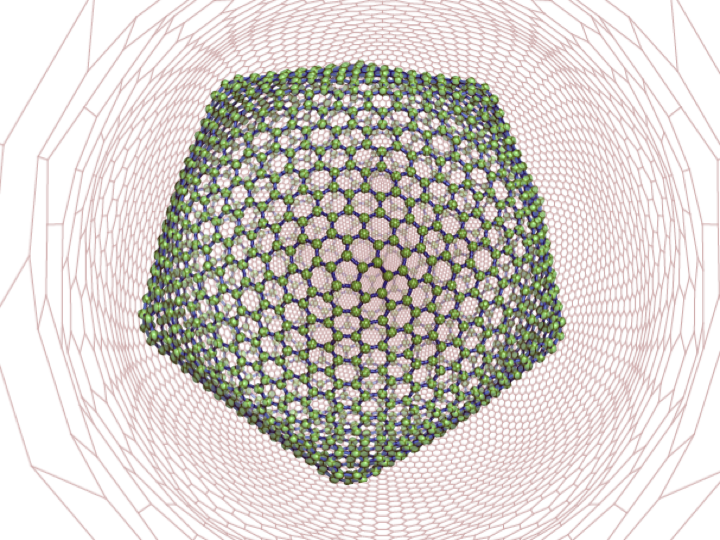
\includegraphics[width=0.6\textwidth]{Toc.png} \\
                 \label{pic:toc}
   	\end{center}
 \end{figure}

\author{Peter Schwerdtfeger}
\email[]{p.a.schwerdtfeger@massey.ac.nz}
\author{Lukas Wirz}\email[]{l.wirz@massey.ac.nz}

\affiliation{Center of Theoretical Chemistry and Physics, The New Zealand Institute
for Advanced Study, Massey University Auckland, Private Bag 102904,
North Shore City, 0745 Auckland, New Zealand.}

\author{James Avery}\email[]{j.e.avery@massey.ac.nz}

\affiliation{Copenhagen, Denmark.}
\date{\today}

\maketitle

\clearpage


{\bf Important Copyright Message:}\\\\
{\it This is an} {\bf open-source code} {\it and you may use and modify the program at your own will.
If you like to know why, read for example} Darrel C. Ince1, Leslie Hatton, 
John Graham-Cumming, Nature {\bf 482}, p.485 (2012). {\it We kindly ask you that if you 
use our program and subsequently publish data to cite the three references given below.
Note: before you distribute the program to other agencies or users outside your
department we kindly ask you pass the information on that new users should be
added to our user database. For details see our website at:}\\
http://ctcp.massey.ac.nz/index.php?group=\&page=fullerenes\&menu=fullerenes.\\\\
For any questions concerning this program please feel free to contact us.
We are always open to improvements and suggestions.\\\\

{\bf Please cite the following papers if you used this program for publishing data:}\\\\
1) P. Schwerdtfeger, L. Wirz, J. Avery, {\it Topological Analysis of Fullerenes - 
A Fortran and C++ Program (Version 4.0)}, (Massey University Albany, 
Auckland, New Zealand, 2012).\\
2) P. W. Fowler and D. E. Manolopoulus, {\it An Atlas of Fullerenes}
(Dover Publ., New York, 2006). This book is highly recommended. 
It helps understanding how this program functions.  Many of the concepts used 
can be found in this book. \\
3) D. Babi\'c, {\it Nomenclature and Coding of Fullerenes}, J. Chem. Inf. Comput. Sci. {\bf 35}, 515-526 (1995).\\\\

{\bf Further reading:}\\\\
4) Z. C. Wu, D. A. Jelski, T. F. George, {\it Vibrational Motions of
Buckminsterfullerene}, Chem. Phys. Lett. {\bf 137}, 291-295 (1987).\\
5) D. E. Manolopoulus and P. W. Fowler, {\it Molecular graphs, point groups, 
and fullerenes}, J. Chem. Phys. {\bf 96}, 7603-7614 (1992).\\
6) G. B. Adams, M. O'Keefe, and R. S. Ruoff, {\it Van der Waals Surface Areas
and Volumes of Fullerenes}, J. Phys. Chem. {\bf 98}, 9465-9469 (1994).\\
7) W. O. J. Boo, {\it An Introduction to Fullerene Structures},
J. Chem. Ed. {\bf 69}, 605-609 (1992).\\
8) D. Babi\'c, D. J. Klein and C. H. Sah, {\it Symmetry of fullerenes},
Chem. Phys. Lett. {\bf 211}, 235-241 (1993).\\
9) T. Pisanski, B. Plestenjak, A. Graovac, {\it NiceGraph Program and its 
applications in chemistry}, Croatica Chemica Acta {\bf 68}, 283-292 (1995).\\
10) B. Plestenjak, {\it An algorithm for drawing Schlegel diagrams}, http://www-lp.fmf.uni-lj.si/plestenjak/Papers/NICEGR.pdf.\\
11) J. Bondy, U. Murty, {\it Graph Theory} (Springer, Berlin, 2008).
12) A. J. M. Wilson, {\it Graphs and Applications. An Introductory Approach} (Springer, Berlin, 2000).\\
13) J. Cioslowski, N. Rao, D. Moncrieff, {\it Standard Enthalpies of Formation of Fullerenes and Their
Dependence on Structural Motifs}, J. Am. Chem. Soc. {\bf 122}, 8265�8270 (2000).\\\\
     
{\bf Acknowledgement}\\\\
PS is indebted to the Alexander von Humboldt Foundation (Bonn) for financial support 
in terms of a Humboldt Research Award, and to both Prof. Gernot Frenking and 
Dr. Ralf Tonner (Marburg) for support during his extended stay in Marburg where 
writing of this program began. We acknowledge the help of Darko Babich, Patrick 
W. Fowler and David E. Manolopoulus to give us the permission to freely distribute 
their Fortran subroutines.\\\\
 
 \begin{figure}[htbp]
   	\begin{center}
  		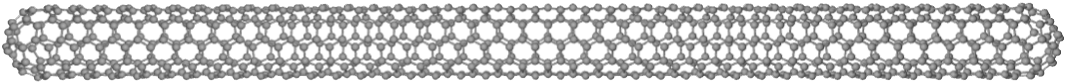
\includegraphics[width=1.0\textwidth]{C840.png} \\
                 \label{pic:toc}
   	\end{center}
 \end{figure}

\clearpage

%Introduction
\section{Introduction}
The Fullerene Program creates cartesian coordinates for different fullerenes isomers and performs a topological/graph 
theoretical analysis of the obtained 3D structure. The results can be used for plotting 2D fullerene graphs (Schlegel diagrams) 
and 3D structures, and as a good starting point for further quantum theoretical treatment. The program was originally 
written in standard FORTRAN and is can easily be implemented in LINUX/UNIX environment. It provides also input files 
to external plotting programs. In the current version only regular fullerene (i.e. consisting of pentagons and hexagons) 
fulfilling Euler's theorem are considered. The program constructs the 3D structure in cartesian coordinates from the 
the canonical ring spiral pentagon indices through either a Tutte embedding (TE) or the adjacency matrix
eigenvector (AME) method. It can also construct the n-th leapfrog and halma fullerenes from
Goldberg-Coxeter transformations of \C{20} or \C{60}. From a general isomer structure one can perform a
Goldberg-Coxeter transformations or one can apply vertex insertions and Stone-Wales transformations. 
The Wu force-field and geometry optimization using a Fletcher-Reeves-Polak-Ribiere
minimization with analytical gradients is implemented in the current version, providing 
a good initial guess for cartesian coordinates. Schlegel diagrams (2D graphs)
can be produced using a variety of different algorithms. The program calculates the volume and surface area 
of a fullerene (irregular or not) through tesselation in trigonal pyramids and calculates measures for
spherical distortion and convexity. It further calculates the minimum covering sphere, the minimum distance sphere
and the maximum inner sphere. Note that in the case of nonplanar 5- or 6-rings there is no unique definition for the 
volume of a fullerene except for the convex hull. There is no reason however why any other definition than the 
fast tesselation algorithm used here should be preferred. The program further calculates the number of Hamiltonian cycles
and produces ring spiral indices. Finally, Cioslowski's scheme for the calculation of the heat of formation for IPR
(independent pentagon rule) fullerenes is implemented \cite{Cioslowski2000}, as well as Babi\'c's scheme for calculating the total resonance energy
of a general fullerene.\cite{Babic1997}\\

This program works for any (distorted or not) regular fullerene (i.e. a fullerene of genus 0 consisting of 
pentagons and hexagons only). The spiral algorithm of Fowler and Manolopoulus used here is not restricted to starting 
from a pentagon or to canonical indices. For a general list of fullerenes see "The House of Graphs" at 
https://hog.grinvin.org/Fullerenes. The program produces a file with default name {\bf cylview.xyz} to be used for plotting 3D 
structures for programs like CYLview \cite{CYLview}, Avogadro, Jmol, or Pymol. Note for using these programs it is important to force-field 
optimize them, otherwise bonds cannot be idendified if structures are used directly from
AME, LME or 3D-TE algorithms (see below). We recommend CYLview, it is more robust and works for the largest 
fullerenes up to 1000 atoms. The program produces fullerene 2D graphs in latex format, but you can
use any other program which is capable of producing Schlegel diagrams, for example
QMGA. For this an input file is written called {\bf qmga.dat} \cite{Gabriel2008}.\\

Version 4.0 (released July 2012) now incorporates C++ routines embedded into the original FORTRAN program using 
much improved algorithms compared to the older version. The reason for using two program languages is
that PS is good in old-fashioned Fortran and JA is good in C++. Also some of the original routines used were available 
in Fortran only. Some standard routines from Mathematical Recipes were modified here for the purpose of matrix diagonalization 
and geometry optimization. This program is under permanent construction. The program has been tested for bugs.
Nevertheless, if you have any problem or find a bug please report to one of us.\\

Not implemented yet and on the to do list (in progress) is:

1) A subroutine to fit the minimum outer ellipsoidal cover useful for  
rugby ball like fullerenes and close packing of ellipsoids (coming soon);

2) Use the general Goldberg-Coxeter construction for fullerenes (coming soon);

3) Geometry optimization using the extended Wu-Fowler force field (coming soon);

4) Frequency calculations from the force field optimized geometry;

5) Construction of non-ring-spiral isomers using the generalized ring spiral algorithm (coming soon);

6) Symmetry labels for H\"uckel orbital energies;

7) Extend to non-regular fullerenes of genus 0 (heptagons and squares);

8) Extend to non-regular fullerenes of genus 1;

9) Symmetrize coordinates to point group symmetry;

10) Restart option for subroutine for Hamiltonian cycle;

11) Use of "House of Graphs" fullerene database (coming soon);

12) Plotting program (other than latex) for producing Schlegel diagrams and corresponding duals (coming soon).


\clearpage
%Installation and running the program
\section{Installation and running the program}
All fortran files are in the directory "source" and all C-files are in the directory "libgraph".
The program is LINUX/UNIX based and works fine with {\bf gfortran} and {\bf gc} compilers. You need to use the Makefile included in 
the fullerene.zip file provided and type\\\\ 
{\bf make}\\\\
It currently compiles in a 64 bit version, but you can change to 32 bits in the Makefile if necessary.
The executable "fullerene" runs on a LINUX/UNIX as\\\\
{\bf ./fullerene $<$inp $>$out}\\\\
A number of test input files can be found in the directory "input". If you type\\\\
{\bf make tests}\\\\
it runs all the input jobs and puts them into *.out in the output directory. If you type\\\\
{\bf make clean}\\\\
all the object files are deleted. More is deleted if you type\\\\
{\bf make distclean}\\\\
If you use the fullerene database, the file needs to be in the directory
where the source and libgraph directories are situated.


\section{Program Structure}
The main program ({\bf main.f}) calls a number of subroutines for certain tasks.
Subroutine {\bf DataIn} manages the input and determines the main tasks to be done.
The input is in {\it Namelist format}. 
Important steps in the program are given in the flow diagram below and are
explained in detain in the following.\\

 \begin{figure}[htbp]
   	\begin{center}
%  		\includegraphics[width=1.0\textwidth]{flowdiagram.png} \\
                 \label{pic:flowdiagram}
        \caption{Flow diagram for main program tasks}
   	\end{center}
 \end{figure}
 
\subsection{Create a 3D structure for a specific fullerene}
The easiest way to create a 3D structure is to read in cartesian coordinates for a specific fullerene 
(see files {\it c20.inp} to {\it c540.inp}), or to construct them internally for the high symmetry 
$Ih-$\C{20} or $Ih-$\C{60} isomers (Subroutine {\bf CoordC20C60}, see input files {\it ico.inp}, {\it icoExp.inp}, {\it icoideal.inp}), or to 
get the cartesian coordinates from input ring spiral pentagon indices (Subroutine {\bf CoordBuild}) by using either the Fowler-Manopoulus 
AME algorithm (the adjacency matrix eigenvector algorithm) \cite{Atlas}, or the more reliable Tutte embedding algorithm (3D-TEA) 
(used by files {\it pentagon1.inp} to {\it pentagon25.inp}). The pentagon indices can also be read-in from the {\it fullerene
database} if the canonical fullerene number is used as defined in The book ``Atlas of Fullerenes" Fowler and Manopoulus \cite{Atlas}.
We recommend reading this book for the use of ring spiral pentagon indices and and H\"uckel (adjacency matrix) $P$-type eigenvectors 
to construct 3D fullerene graphs. Note it is critical to get the right H\"uckel eigenvectors for the construction of cartesian coordinates. 
The 3 $P$-type vectors may need to be read in (see file {\it pentagon8.inp} for such an example).
If the AME algorithm fails you can use our Tutte embedding algorithm (which to our opinion is less troublesome 
and may be used as the standard method to construct 3D structures). It is important that the end-product is 
viewed by a molecular visualization program. We recommend CYLview by Claude Legault \cite{CYLview},
Avogadro \cite{Avogadro}, JMol \cite{JMol} or Pymol \cite{Pymol}. These codes are all freely downloadable.
For this purpose a file is written out to cylview.xyz to be used as an input file for these programs. 
The program sets barycenter of the fullerene 
to the origin. Using these coordinates the program calculates the smallest and largest cage diameters which gives already a measure 
for distortion from spherical symmetry (Subroutine {\bf Diameter}). It produces the distance matrix if print level 
is set to high (Subroutine {\bf DistMatrix}), and once the point group is obtained the program determines if the
fullerene is chiral or not (Subroutine {\bf Chiral}).\\

The program can print all general and IPR isomers for a specific fullerene and perform an analysis introduced 
mostly in the book by Fowler and Manolopoulus \cite{Atlas}, e.g. pentagon indices and 
pentagon number, hexagon indices and strain parameter, NMR information and number of distinct Hamiltonian cycles if 
required. Note that the number of isomers scale polynomially to the 9th power, thus it becomes soon computationally
too demanding beyond \C{100}. Moreover, the database can be used to print all isomers up to \C{100} and up to \C{120}
for all IPR isomers.\\


Once the cartesian coordinates are known, all edges are determined by analyzing connectivities between vertices from either given cartesian
coordinates or from adjacency matrix if a ring spiral input was used (Subroutine {\bf Connect}). In any case
one has the adjacency matrix $A_{ij}$ for all vertices and edges at this stage.
From $A_{ij}$ a H\"uckel analysis is performed (Subroutine {\bf Hueckel}). This gives you a good hint if the 
fullerene is open or closed shell. Note that for fullerenes the H\"uckel analysis may not be very reliable 
as hybridization with the C(2s) orbitals occur due to nonplanarity. Hence the $\sigma-\pi$ separation breaks down
especially for the small fullerenes. Nevertheless, we adopt $\alpha$=-0.21 au  and  $\beta$=-0.111 au obtained
from the exp. ionization potential (7.58 eV) and excitation energy (3.02 eV) of \C{60} (note the electron goes 
into the second LUMO of $t_{1g}$ symmetry). This gives also orbital energies for \C{60} in reasonable 
agreement with DFT Kohn-Sham orbital energies. The fullerene might also Jahn-Teller distort adopting a singlet 
ground state instead of one of a higher multiplicity as this is the case for \C{20}. Such electronic effects are not
captured in this program, and one needs to perform a proper quantum theoretical calculation. The total resonance energy
is calculated from Babi\'c's fit data \cite{Babic1995,Babic1997}.\\

In a next step a Goldberg-Coxeter transformation $GC_{k,l}(n)$ for a fullerene \C{n} can be performed if required from input
(Subroutine {\bf GoldbergCoxeter}). This leads to a fullerene C$_{k^2+kl+l^2}$. The current implementation allows only for
{\it leapfrog transformations} ($k=l=1$) and for {\it halma transformations} ($k \neq 0$ and $l=0$). The program allows for multiple leapfrog
transformations for the construction of very large fullerenes. A general $GC_{k,l}(n)$  for all values of $k$ and $l$ is in
preparation.\\

Subroutine {\bf Hamilton} uses the back-track algorithm of Babi\'c \cite{Babic1995a} to obtain all 
Hamiltonian cycles and subsequently the IUPAC name of the fullerene. The number of Hamiltonian cycles given has been checked 
against a second algorithm. Note, the number gives all distinct Hamiltonian cycles and left-right cycles counted as the 
same. Although finding all Hamiltonian cycles is a NP-complete problem, it works fine up to about \C{100}. 
After that it becomes computationally too demanding. The program therefore prints upper and lower limits instead
for the larger fullerenes. The existence of Hamiltonian cycles for fullerenes is only conjectured, and only for layered fullerenes 
(e.g. fullerene with onion-shaped 2D graphs such as nanotubes) it has been proven to exist. Our calculations proved that
they exist for all fullerene isomers up to \C{100} and all IPR isomers up to \C{120}.\\

The geometry can be optimized by force fields using a Fletcher-Reeves-Polak-Ribiere geometry optimization with analytical 
gradients (Subroutine {\bf OptFF}). At the moment only the Wu force field is implemented which considers bond lengths and
angles in an harmonic oscillator approximation \cite{Wu87}. It is very fast though, even for fullerenes such as \C{840}. 
Note that the Wu force-field optimization might distort the fullerene from the ideal point group symmetry. Moreover, as no
dihedral angles are confined, the molecule might distort away from convexity. In such a case a Coulomb repulsive potential can
be added (see input instructions). Note that the construction of the fullerene by using the AME or Tutte algorithm may
lead to a more spherical arrangement, e.g. barrels instead of nanotubes. More sophisticate force fields are being
developed currently.\\

Subroutine {\bf Ring} identifies all closed 5- and 6-ring systems (faces) and determines if Euler's theorem is fulfilled.
Subroutine {\bf RingC}) then determines the center for each 5- and 6-ring later used for the trigonal pyramidal tessellation to obtain
the volume and surface. This routine also analyzes all 2- and 3-ring fusions and many other useful patterns needed for example
in Stone-Wales transformations or vertex insertions. It further determines the Rhagavachari-Fowler-Manolopoulos neighboring pentagon 
and hexagon indices as described in detail in Fowler and Manolopoulos' book \cite{Atlas}.
From the hexagon indices one derives if the fullerene is IPR or not. If it is IPR, Cioslowski's scheme is used to calculate the 
heat of formation \cite{Cioslowski2000}.\\

Information from the subroutine {\bf RingC} is used to perform Stone-Wales transformations (subroutine {\bf StoneWalesTrans}), Endo-Kroto
2-index insertions (subroutine {\bf EndoKrotoTrans}, Yoshida-Fowler 4-vertex ($D_{3h}$ 6555) (subroutine {\bf YoshidaFowler6}) and 6-vertex ($D_{3h}$ 666555) 
insertions (subroutine {\bf YoshidaFowler6}), or the WS 6-vertex (6-55-55) insertion if required. The non-spiral fullerenes such 
as  \C{380} or  \C{384} can be constructed with these vertex insertion methods.\\

(Subroutine {\bf SpiralSearch}) uses ring-spiral algorithm of Fowler and Manopoulus for the search of a ring spiral if for the input
cartesian coordinates were chosen of the fullerene was modified. It produces canonical ring spiral pentagon indices if the fullerene is spiral.\\

The volume and surface area of the fullerene is calculated in Subroutine {\bf Volume}. This is done by 
summing over all tetrahedrons spanned by the three vectors CM-CR  (barycenter of fullerene to the ring center),
CM-CA1 (barycenter of fullerene to atom 1 in ring), and CM-CA2 (barycenter of fullerene  to atom 2 in ring).
There are 5 such tetrahedrons in a pentagon and 6 in a hexagon. Note that the barycenter CM is already set to the origin.
In a similar way the surface area is obtained by summing over all triangles from the ring center to neighboring vertices in the ring.
$I_h$-\C{20} and $I_h$-\C{60} coordinates can be constructed easily using basic geometry. For these the volume and surface areas are
known analytically. The routine also calculate the exact volume through a different tesselation method .... Also the convex hull
is constructed.\\

Three routines follow to calculated the minimum covering sphere (MCS) of a fullerene (Subroutine {\bf MinCovSphere2}) using the second
algorithm of Yildirim \cite{Yildirim08,Hopp96}, minimum distance sphere (MDS) (Subroutine {\bf MinDistSphere}), and the maximum inner sphere (MIS)
(Subroutine {\bf MaxInSphere}). The MCS in $m$-dimensional space is uniquely defined can be expressed as a convex combination of at most 
($m$+1) points, hence our algorithm stops when 4 points are left over in the iteration process of the algorithm.
Note: The spherical central cover SCC is not the minimum covering sphere MCS
(except if all distances from the center of points CM are the same as in the
ideal capped icosahedron). The spherical central cover is taken from the
CM point with radius Rmax (longest distance to one vertex). Note that we changed the first
condition in this Yildirim's algorithm by choosing the furthest point from CM.
In the final statistics there should be 0 points outside the sphere and at least 1 point on the sphere.
At the end the Van der Waals radius of carbon (1.415 \AA) is added to the radius of the minimum covering sphere 
(note input coordinates for this need to be in \AA otherwise change the program), and the volume of
an ideal fcc solid is calculated. The Van der Waals radius is chosen such that
for \C{60} the solid-state results of Heiney et al. \cite{Heiney91}
are reproduced. The definition of the distortion parameter $D$ from the MCS or for the isoperimetric quotient IPQ is
$IPQ=36Pi(V^2/A^3)$. D=[100/(N*Rmin)]* sum(i=1,N) {Rmcs - ||pi-Cmcs|| }    (N=MAtom).\\

The minimum distance sphere (MDS) of the fullerene is biased for the case that few atoms stick 
out on a sphere and the MDS measure may be more appropriate for a measure from spherical distortion. The MDS is defined as
The problem can be reduced to min(Cmds) 1/N sum(i=1,N) | Rmds - || p(I) - Cmds || |
where ||..|| is the Eucledian norm in m dimensions. Cmds has to lie within the
convex hull. The MDS may not be uniquely defined, as there can be many 
(even degenerate) local minima, but for most spherical fullerenes it should 
just be fine. Analogous to the MCS there will be a measure for distortion from spherical symmetry.
D=[100/(N*Rmin)]* sum(i=1,N) | Rmds - || p(I) - Cmds || |\\

The maximum inner sphere (MCS) of the cage molecule
max(Cmds) min(i) || p(I) - Cmds ||
The maximum inner sphere is important for evaluating how much space
there is in a fullerene for encapsulating atoms and molecules. For
this the radius and volume is printed out with the Van der Waals
radius of carbon taken off Rmds. 

Finally, produce the (X,Y) coordinates of a fullerene graph (Subroutine SCHLEGEL).
Schlegel projection (SP):
Here the points are rotated (if in input I1,I2, and I3 are given) so to
put the selected vertex, edge or ring center on top of the z-axis as the
point of projection (otherwise the point (0,0,zmax) is chosen with zmax
being the point with maximum z-value from the original input coordinates).
Points are then sorted in descending order according to their z-values.
The circumference for atoms and rings down the z-axis are determined.
The Schlegel projection is created giving as output the projected (X,Y)
coordinates. The connections between the points are already written out
earlier in the output such that the fullerene graph can be drawn.
There are two choices for the projection, depending if you choose the
outer ring or the center part of the fullerene graph as a starting point:
    
1) The cone projection (CSP), i.e. points are projected out to an enveloping 
       cone and then down to a plane below the fullerene. The input I1,I2,I3 
       defines the center of the fullerene graph. The last ring center should 
       be at the bottom of the fullerene and if detected, will not be projected 
       out, or if not will have a large scale factor (this center may be ignored 
       in the drawing). Also, the last points on the outer ring in the fullerene
       graph are scaled in distance by 1.2 in order to make the outer rings 
       more visible. This also moves the outer centers within the ring.

2) The perspective projection (PSP), i.e. points are projected down a plane 
       from a set projection point. In this case the input I1,I2,I3 defines the
       peripheral ring of the Schlegel diagram. 
       
At the end a rough printout of the fullerene graph is produced. Note that this is o.k for fullerenes up to about \C{100}, beyond it
it becomes too crowded and a proper plotting program should be used. Nevertheless, it serves for a first rough picture. 
Furthermore, for large fullerenes it becomes critical to correctly set the projection point or point of the cone. If for example the projection
point is too far away from the fullerene, edges may cross.
Other algorithms for producing Schlegel diagrams:
    
3) Tutte graph with linear scaling (2D-TGE-LS)

4) Spring embedding with barycentric Coulomb repulsion (SE+C)
     
5) Pisanski-Plestenjak-Graovac embedding (PPGA)
 
6) Kamada-Kawai embedding (2D-KKE, this gives a 2D picture of a 3D structure
and has edge crossings).
    
You should also be aware of program fullgen for generating nonisomorphic fullerenes.
It is written by Gunnar Brinkmann (Gunnar.Brinkmann@Ugent.be) and can be
downloaded from Brendan McKay's website (Australian National University) at
http://cs.anu.edu.au/~bdm/plantri/
   
The time consuming steps in the program are the adjacency matrix diagonalization needed for the AME algorithm, the force-field optimization for very large
fullerenes ($>$ 2000 atoms), the determination of the number of Hamiltonian cycles ($>$ 80 atoms), and the number of isomers ($>$ 80 atoms),
and the Tutte embedding algorithm ($>$ 2000 atoms).


%Input description
\section{Input description}

Input and output files are in the folders  input  and   output  respectively. This program has been tested for the ideal capped 
icosahedron \C{60} ({input files ico.inp) and for many other fullerenes which are found in the following input files:
\C{20} (c20.inp), \C{24} (c24.inp), \C{26} (c26.inp), \C{28} (c28.inp), \C{30} (c30.inp),
\C{36} (c36.inp), \C{50} (c50.inp), \C{60} (c60.inp), \C{70} (c70.inp), \C{72} (c72.inp),
\C{74} (c74.inp), \C{78} (c78.inp), \C{80} (c80.inp), \C{92} (c92.inp), \C{100} (c100.inp),
\C{180} (c180.inp), \C{320} (c320.inp), and \C{540} (c540.inp), pentagon1.inp, ..., pentagon25.inp
The coordinates used in the input files are mostly B3LYP aug-cc-pVDZ optimized up to \C{60}, and cc-pVDZ up to \C{180}, 
and 6-31G for the rest and all for singlet states (except of course for the ones where the pentagon indices input is
chosen). Note that for some of the fullerene coordinates the singlet state chosen may not be the electronic ground state.
Many definitions depend on the use of {\AA}ngstr{\o}ms for distances, so please use this unit. A typical input is in {\it Namelist format},
or if additional data are required in free format, and read like this:\\\\
C80  Using FM algorithm to produce coordinates, pentagon12.inp \\
\&Coord NA=80, IC=2, IV2=4, IV3=5 / \\
\&FFChoice Iopt=1 / \\
\&FFParameters / \\
\&Hamilton IHam=1 / \\
\&Isomers IPR=1 / \\
\&Graph ISchlegel=2, ISO1=2, ISO2=4, ISO3=5 / \\
1 2 3 4 5 6 37 38 39 40 41 42 \\

The first line is a text line, the second \&Coord line in namelist format tells the program how the coordinates are created (and many more), the
next two lines \&FFChoice and \&FFParameters are specifications for the force field to be used (none in this case), line 4 (\&Hamilton) concerns the
Hamiltonian cycles, line 5 (\&Isomers) is an isomer list is created, and line 6 (\&Graph) for the 2D fullerene graph (Schlegel diagram). The last
line in the input for the 12 pentagon ring-spiral indices.

In the following the input in the required sequence is described in detail (either Namelist or in Free Format):\\\\

1) Text line of 80 characters (in A132 format) (you can put as many text cards in as you want)\\\\

2) {\bf \&Coord line}: Input to create cartesian coordinates and main flags for the program (e.g. \&Coord IC=20, IOPT=1, R6=1.42 /).\\
List of options:\\ 
{\bf NA, IC, IV1, IV2, IV3, ixyz, isonum, kGC, lGC, IP, IPRC, leap, leapGC, ihueckel, ISW, KE, loop, mirror, IYF, IWS, ichk, TolR, R5, R6, xyzname}\\
NA= Number of Atoms (Default: 60)\\
IC= Flag for the construction of the 3D structure (cartesian coordinates) (Default: 0)\\
IP= Print option (Default: 0)\\
IV1= Number for H\"uckel P-type eigenvector for AME algorithm (Default: 2)\\
IV2= Number for H\"uckel P-type eigenvector for AME algorithm (Default: 3)\\
IV3= Number for H\"uckel P-type eigenvector for AME algorithm (Default: 4)\\
ixyz= Flag for producing input file for CYLview, Avogadro or others in standard xyz format (Default: 0)
isonum= Isomer number according to the scheme of Fowler and Manopoulus (Default: 0).
If IC=2, 3 or 4 and isonum not zero, than pentagon indices are taken from the isomer list contained in a database (see below). 
There are two databases, one for the general isomers (IPRC=2) and one for the IPR isomers (IPRC=1), the
definition is similar to the IPR parameter below (Default: 2).\\
TolR= Tolerance in \% (Default: 33).\\
R5= pentagon bond distance, i.e. the bond length in the pentagons (Default: 1.455).\\
R6= hexagon  bond distance, i.e. the bond length of the bonds connecting hexagons (Default: 1.391).  
If R5=R6 is chosen then the ideal capped icosahedron for \C{60} is obtained if NA=60 is chosen.\\
xyzname=filename (max 20 characters) if ixyz.ne.0 (default: cylview.xyz).\\\\

Details for the {\bf IC}-flag:\\
If IC = 0 No coordinate input required, coordinates are constructed for the IPR isomer of \C{60} (or \C{20} if NA=20 is chosen).
You may like to specify R5 and R6 in the input, otherwise the default values are taken.\\
If IC = 1 Cartesian Coordinates expected as input. In this case NA extra lines are required with\\\\
$N_{Z_i}, X_i, Y_i, Z_i$  (in free format)\\\\
Here $N_{Z_i}$= Nuclear Charge, and X,Y,C are the cartesian coordinates for atom $i$ in \AA. NB: $N_{Z_i}$ is not really needed by the program, 
but you can copy easily .xyz files or outputs from other quantum theoretical programs into the input.\\
If IC = 2 or 3 the adjacency matrix is created from a ring-spiral pentagon list. Extra input required (free format):\\\\
$n_{RSPI}(I), I=1,12$ \\\\
$n_{RSPI}(I)$ are the 12 Fowler-Manolopoulus ring-spiral pentagon indices which uniquely identify the locations of the 
pentagons if the fullerene is spirable \cite{Atlas}. Use the canonical pentagon ring indices if possible (transformation to the canonical
from should work as well).\\
If IC = 4 or 5 adjacency matrix is created from a Goldberg-Coxeter transform of \C{20}, i.e. $GC_{k,l}$[\C{20}]. Note at the moment
the program is restricted to $l=0$. In this case the parameter kGC in the namelist input has to be used.\\
If IC = 2 or 4 the AME algorithm using $P$-type eigenvectors produced from the adjacency matrix to get cartesian coordinates. 
If the $P$-type eigenvectors are not in sequence
(position 2,3 and 4, see ref.\cite{Atlas} for details), three integer values $I_{V_1}, I_{V_2}, I_{V_3}$ can be specified in the \&Coord
namelist input identifying the position of the eigenvectors (see pentagon8.inp for such an example).
In this case a warning occurs which means you should carefully check the eigenvectors used and cartesian coordinates produced.
Otherwise coordinates produced are useless. This is more often the case as you might expect.\\
IC = 3 or 5 the Tutte embedding (3D-TE) algorithm is chosen for the construction of the 3D fullerene structure from the adjacency matrix. 
This should always work,
although the fullerene created might be too spherical compared to the AME algorithm. But this algorithm is easier, and (in theory) 
should never fail. Examples are given in the input files starting with ``pentagon".\\
If IP $>$ 0 a larger output produced, i.e. the full distance matrix, all Hamiltonian cycles and all 3-ring connections.\\
TolR: Only change this parameter if the program cannot produce correctly the adjacency matrix. This is only necessary for the cartesian
coordinate input (IC=1) and only fails if bond distances are unusually large or small. Connectivities are found for atoms with distances between
R6   and   R6*(1+TolR/100). If TolR=0.0 the default value of 33\% is used. If this parameter is set at a value too large, unwanted connectivities
are produced resulting in smaller polygons. This parameter should reflect the maximum deviation in distance from the smallest distance found.\\
 
if leap=n than the n-th leapfrog fullerene is generated.\\\\

3) {\bf \&Opt line}: Option for force-field optimization:
      \&Opt options /        (e.g. \&Opt Iopt=1 /)
      list of options: Iopt,ftol,WuR5,WuR6,WuA5,WuA6,WufR,WufA,fCoulomb
      Iopt= Flag for force-field optimization (Default: 0)
      In detail:
       If Iopt=1  then fullerene is optimized using the force field method
         of Wu et al within a Fletcher-Reeves-Polak-Ribiere algorithm:
         Z.C.Wu, D.A.Jelski, T.F.George, Chem. Phys. Lett. 137, 291-295 (1987).
         Note that there are more sophisticated force fields available,
         but for these general parameters for fullerenes are not
         yet available, and the Wu force field does the job to create good initial
         cartesian coordinates for further refinement using more sophisticated
         QM methods. Note that a converged energy much greater than zero implies
         that the set distances and angles in the Wu force field cannot be
         reached for all atoms and rings. For further reading see: 
         A.Ceulemans, B.C.Titeca, L.F.Chibotaru, I.Vos, P.W.Fowler, 
         J. Phys. Chem. A 105, 8284-8295 (2001).
       If Iopt=2  Preoptimize with input force field, then optimize with Wu
         force field. This is especially useful for fcoulomb input (see below).  
         NB: Avogadro has a more sophisticated force-field which you can try out.
       ftol: The convergence tolerance on the function value is input as ftol
         (Default: 5.0E-8)
       WuR5,WuR6,WuA5,WuA6,WufR,WufA: Force field parameters for Wu force field for
         distances R5, R6, angles A5, A6, force constants for distance WufR and
         angles WufA (see paper by Wu et al. for details).
         Defaults: WuR5=1.455, WuR6=1.391, WuA5=1.08d2, WuA6=1.2d2, WufR=1.d6,
                   WufA=1.d5
       If fCoulomb>0. then add an additional repulsive Coulomb forct from the 
         barycenter to the atoms      (Default:  fCoulomb=0.d0)
         This is extremely useful for an initial geometry optimization to keep
         the cage convex if for example the Tutte construction leads to not
         a good guess of the initial structure. In such cases fCoulomb=1.d2
         is a good choice.\\\\

 4) Option for calculating Hamiltonian cycles and IUPAC numbers 
      \&Hamilton options /        (e.g. \&Hamilton IHam=1 IUPAC=1 /)
      list of options: IHam,IUPAC
      In detail:
      If IHam>0 Then Subroutine HAMILTON is called.     (Default: 0)
         IHam=1 Routine will stop after 1 million Hamiltonian cycles are found
         IHam=1000000000 Program runs forever and prints if IHam is reached
      If IUPAC=1 IUPAC numbers are produced.   (Default: 0) 
         Note only with this option together with IP=1 in \&Coord input 
         all Hamiltonian cycles are printed out. IP=0 only gives the
         best cycle (see Babic, ref.3).
         IUPAC=0 goes into a fast subroutine and prints only the total number of
         Hamiltonian cycles.\\\\

 5) Option for producing list of isomers and properties.
      \&Isomers options /        (e.g.\&Isomers IPR=1, IPH=1 /)
      list of options: IPR,IPH,IStop,IChk,chkname (Default 0 for all options
                                                   and 'checkpoint' for chkname)
      In detail:
      If IPR>0 then the ring spiral subroutine of Fowler and Manolopoulus is used.
         This sub-program catalogues fullerenes with a given number of
         vertices using the spiral algorithm and a uniqueness test
         based on equivalent spirals. The required input is IPR.
         IPR=1 for isolated-pentagon isomers from C60 onwards.
         IPR=2 for general isomers (note that this generates a lot of output and
            takes some computer time for fullerenes larger than C60).
      If IPH=1 then number of distinct Hamiltonian cycles is calculated for
          every isomer (note this is computer time extensive).
      If istop=1 program stops after calling this routine.
      If IChk=1  Restart: Isomer list is continued from previous output file 
          called 'checkpoint' as default if not otherwise give in chkname.
          This is a restart option from a previous run which terminated. Note
          that the new output file does not contain the previous one.
      The resulting output is a catalogue of the isomers found containing
         their idealized point groups, canonical spirals, and NMR patterns
         (see ref.2).\\\\

 6) Option for producing coordinates for fullerene graphs (Schlegel diagrams).
      \&Graph options /      (e.g. \&Graph IG=1, ISO1=1, ISO2=3, ISO3=7 /)
      list of options: ISchlegel,ISO1,ISO2,ISO3,PS,SCALE,SCALEPPG
      We recommend IG= 1, 2, 4 or 7
      In detail:
      If ISchlegel>0 Use Program Schlegel for generating fullerene graphs
         ISchlegel=1 Use the perspective projection method (PSP).
         ISchlegel=2 Use the cone projection method (CSP).
         ISchlegel=3 Produce the Tutte graph (2D-TE)
         ISchlegel=4 Produce the Tutte graph and perform linear scaling (2D-TE-LS)
              (scale factor can be read in).
         ISchlegel=5 Produce the Tutte graph and perform spring embedding optimization
              (rij-r0)**2 with r0 set to 2.0 (2D-SE).
         ISchlegel=6 Starting from the Tutte graph perform spring + repulsive Coulomb
              force embedding optimization (2D-SE+C). The repulsive force is taken
              from the barycenter to the vertex. r0 is set to 2.0. The force
              constants are set such that the graph looks nice.
         ISchlegel=7 Starting from the Tutte graph perform a Pisanski-Plestenjak-Graovac 
              embedding PPGE) optimization (called Schlegel by the authors)
              Note: This is much faster than their simulated annealing algorithm.
         ISchlegel=8 Starting from the Tutte graph perform a Kamada-Kawai embedding 
              optimization using the distance matrix (2D-KKE).
              Note: This gives a 2D picture of a 3D structure, thus
               it is not related to a Schlegel diagram and has edge crossings.
      If ISO1=0 Use the input coordinates for the construction of 
               the Schlegel diagram.
      If ISO1.ne.0 Specifying the ring center, edge or
              vertex through which the z-axis goes at the top of
              the projection (under construction). This rotates
              the fullerene around the origin of points into the
              right position for the Schlegel diagram. Since 3 atoms
              uniquely define the ring, two the edge, and one the vertex,
              the input is three integers with the corresponding
              atom numbers  IO1, IO2, and IO3, i.e. for these values
                    1 0 0 is a vertex with atom 1 on the top of the z-axis;
                    7 8 0 is an edge between atom 7 and 8 and z-axis goes
                          the middle of the bond;
                    12 13 50 is a ring (either pentagon or hexagon determined
                          by the program) and z-axis goes through the center
                          of the ring;
              NB: You can run the program first with 0 0 0, check the positions
                  and run it again with the appropriate values.
              NB2: For IG=1 the input (if chosen) requires to be a ring, i.e.
                  IO1, IO2 and IO3 are required, otherwise they are chosen by the
                  program using the largest z-coordinate.
      If Scale.ne.0. Scaling factor for linear scaling of Tutte graph (default  2.5)
              2D coordinated are scaled by 1.+.5*Scale*(rmin-r)/rmin
              r is the distance of the vertex from the barycenter
              rmin is the smallest distance of the vertex from the barycenter 
               belonging to the outer circumferencing 5- or 6-ring
      If ScalePPG.ne.0. Scaling factor for exponential in Pisanski-Plestenjak-Graovac
              algorithm     (default 1.0)
      If PS.ne.0. 
              - Projection angle in degrees is chosen (default 45 degrees)
              to be used as an input parameter in the cone projection
              method. The angle is the cone angle from the point of projection 
              to the projection plane, which touches the point with the smallest 
              z-value (opposite the projection point). Note that angle is reset 
              to 45 deg if chosen larger than 89.
              - In the case of the perspective projection PS is the distance
              between the focal point and the ring center underneath, Note this
              is chosen by the program, but if nonzero this parameter has to be
              carefully chosen. The picture produced gives a good idea if the
              ParamS is correctly chosen or not. Note that the ring centers get
              an extra boost of 10\% in the scaling factors such that they appear
              more in the center of the rings produced by the Schlegel projection.
              
\section{Fullerene Isomer Database}
A database is provided for general isomers up to \C{100} and for IPR isomers up to
\C{120} including the number of Hamiltonian cycles. The database can be copied into
the main program folder and can be used to read the ring spiral pentagon indices.
The numbering scheme is identical to that the one chosen in the book by Fowler 
and Manolopoulus,\cite{Atlas}, that is each isomer in the book's appendix can be 
constructed easily from the database. An example is given in the input file   
{\it pentagon13.inp}. The datafiles are formatted and can easily be read. It is our 
intension to extend the isomer list beyond \C{100}/\C{120} (without Hamiltonian cycles). 
New lists will be available on our website. Note the determination of the number of
distinct Hamiltonian cycles is NP-complete and beyond 100 (120 for IPR) 
computationally too demanding. The longest file for our database ran for 3
months on a single processor.
Note: the directory database needs to be in the same directory as ``source" or ``libgraph".


%References

\begin{thebibliography}{35}

\bibitem{CYLview} C. Y. Legault, ``Program CYLview", http://www.cylview.org. 

\bibitem{Gabriel2008} A. T. Gabriel, T. Meyer, and G. Germano, 
``Molecular graphics of convex body fluids", {\it J. Chem. Theory Comput.}
{\bf 4}, 468--476 (2008). The program is available at http://qmga.sourceforge.net/.

\bibitem{Cioslowski2000} J. Cioslowski, N. Rao, D. Moncrieff, "Standard Enthalpies of Formation of Fullerenes and Their
Dependence on Structural Motifs", {\it J. Am. Chem. Soc.} {\bf 122}, 8265�8270 (2000).

\bibitem{Babic1995} D. Babi\'c, O. Ori, ``Matching polynomial and topological resonance energy of \C{70}", {\it Chem. Phys. Lett.} {\bf 234}, 240-244 (1995).

\bibitem{Babic1997} D. Babi\'c, ``Topological Resonance Energy of Fullerenes", {\it J. Chem. Inf. Comput. Sci.} {\bf 37}, 920-923 (1997).

\bibitem{Atlas} P. W. Fowler and D. E. Manolopoulus, ``An Atlas of Fullerenes" (Dover Publ., New York, 2006).
 
\bibitem{Avogadro} see http://avogadro.openmolecules.net

\bibitem{JMol} see http://jmol.sourceforge.net/

\bibitem{Pymol} see

\bibitem{Babic1995a} D. Babi\'c, ``Nomenclature and Coding of Fullerenes", {\it J. Chem. Inf. Comput. Sci.} {\bf 35}, 515-526 (1995).

\bibitem{Wu87} Z. C. Wu, D. A. Jelski, and T. F. George, ``Vibrational Motions of
Buckminsterfullerene", {\it Chem. Phys. Lett.} {\bf 137}, 291-295 (1987).

\bibitem{Yildirim08} E. A. Yildirim, {\it SIAM Journal on Optimization}, {\bf 19}, 1368-1391 (2008) 

\bibitem{Hopp96} T. H. Hopp and C. P. Reeve, NIST, US Department of Commerce (1996).

\bibitem{Heiney91} P.A.Heiney et al., Phys. Rev. Lett. 66, 2911 (1991)

\end{thebibliography}

\end{document}

